\documentclass[a4paper,9pt]{report}
\usepackage[utf8]{inputenc} %du mettre utf8 et pas utf8x car incompatible avec biblatex
\usepackage{graphicx}
\usepackage{tikz}
\usepackage{forest}
\usepackage{pgfplots}
\usepackage{xcolor}
\usepackage{colortbl}

\usepackage{tgtermes}
\usepackage{lmodern}
\usepackage{amsmath}


\usepackage[
pdftitle={PROJ0016 | Project Review \#1},
pdfauthor={Céline BAUDENNE, Arnaud DELAUNOY, Francois CORNET},
colorlinks=true,linkcolor=blue,urlcolor=blue,citecolor=blue,bookmarks=true,
bookmarksopenlevel=2]{hyperref}
\usepackage{mathtools,amssymb,amsthm,textcomp}
\usepackage{enumerate}
\usepackage{multicol}
\usepackage{multirow}
\usepackage{listings}
\usepackage{color} %red, green, blue, yellow, cyan, magenta, black, white
\definecolor{mygreen}{RGB}{28,172,0} % color values Red, Green, Blue
\definecolor{mylilas}{RGB}{170,55,241}


\usepackage{tikz}
\usetikzlibrary{trees}

\usepackage{geometry}
\geometry{total={210mm,297mm},
left=20mm,right=20mm,%
bindingoffset=0mm, top=20mm,bottom=20mm}

%add bibliography
%\usepackage[backend=biber]{biblatex}
%\addbibresource{biblio.bib}


\linespread{1.3}


\newcommand{\linia}{\rule{\linewidth}{0.5pt}}
\renewcommand{\thesection}{\arabic{section}}

% custom theorems if needed
\newtheoremstyle{mytheor}
    {1ex}{1ex}{\normalfont}{0pt}{\scshape}{.}{1ex}
    {{\thmname{#1 }}{\thmnumber{#2}}{\thmnote{ (#3)}}}

\theoremstyle{mytheor}
\newtheorem{defi}{Definition}

% my own titles
\makeatletter
\renewcommand{\maketitle}{
\begin{center}
\vspace{2ex}
{\huge \textsc{\@title}}
\vspace{1ex}
\\
\linia\\
\@author \hfill \@date
\vspace{4ex}
\end{center}
}
\makeatother
%%%

% custom footers and headers
\usepackage{fancyhdr,lastpage}
\pagestyle{fancy}
\lhead{}
\chead{}
\rhead{}
\lfoot{PROJ0016 - Big Data Project |  Project Review \#1}
\cfoot{}
\rfoot{Page \thepage\ /\ \pageref*{LastPage}}
\renewcommand{\headrulewidth}{0pt}
\renewcommand{\footrulewidth}{0pt}
%

%%%----------%%%----------%%%----------%%%----------%%%
\begin{document}

\begin{titlepage} % Suppresses displaying the page number on the title page and the subsequent page counts as page 1
	\newcommand{\HRule}{\rule{\linewidth}{0.5mm}} % Defines a new command for horizontal lines, change thickness here

	\center % Centre everything on the page

	%------------------------------------------------
	%	Headings
	%------------------------------------------------

	\textsc{\LARGE University of Liège}\\[1.5cm] % Main heading such as the name of your university/college

	\textsc{\Large Big Data Project}\\[0.5cm] % Major heading such as course name

	\textsc{\large PROJ0016}\\[0.5cm] % Minor heading such as course title

	%------------------------------------------------
	%	Title
	%------------------------------------------------

	\HRule\\[0.4cm]

	{\huge\bfseries Project Review \#1 - Pre-analysis and Literature review}\\[0.4cm] % Title of your document
	\HRule\\[1.5cm]

	%------------------------------------------------
	%	Author(s)
	%------------------------------------------------

	% If you don't want a supervisor, uncomment the two lines below and comment the code above
	{\large\textit{Authors}}\\
  Céline \textsc{BAUDENNE}\\
  Arnaud \textsc{DELAUNOY}\\
	François \textsc{CORNET}


	%------------------------------------------------
	%	Date
	%------------------------------------------------

	\vfill\vfill\vfill % Position the date 3/4 down the remaining page

	{\large October 29th 2018} % Date, change the \today to a set date if you want to be precise

	%------------------------------------------------
	%	Logo
	%------------------------------------------------

	%\vfill\vfill
	%\includegraphics[width=0.2\textwidth]{placeholder.jpg}\\[1cm] % Include a department/university logo - this will require the graphicx package

	%----------------------------------------------------------------------------------------




	\vfill % Push the date up 1/4 of the remaining page

\end{titlepage}


\section{Problem Formalization}
\subsection{Tournament model}
A tournament can be seen as a tree, as illustrated in Figure~\ref{fig:tree}. A given depth in the tree corresponds to a given round
in the tournament. Each node corresponds to a player.
The leaves correspond \textit{directly} to players while intern nodes correspond to
the winner of the match between their two children.

The probability that Player $i$ beats Player $j$ is given as $M_{i,j}$.
One denotes the probability that Player $i$ wins and reaches round $r$ as $R_{i,r}$.
This probability is given by the product between the probability of reaching round $r-1$
and the probability of beating their opponent at this round.
Formally, it can be expressed as follows:
\begin{equation}
  \begin{cases}
    R_{i,r} = R_{i,r-1} \left(\sum_{j \in J}M_{i,k}R_{j, r-1} \right) & \text{with $r > 0$}\\
    R_{i,0} = 1
  \end{cases}
\end{equation}
Except at round $1$, Player $i$ does not know in advance who the opponent is going to be. 
What is already \textit{known} is that a given Player $j$ has a probability $R_{j, r-1}$ to reach the round $r-1$ and that Player $i$ has a probability $M_{i,j}$ to beat Player $j$.

One now has to determine which players could meet Player $i$ at round $r$, in other
words the range of players indexes $J$.
Since when Player $i$ reaches round $r$, all other players of the same
subtree were eliminated, the range may not include the ones of this subtree.
It consists then in taking all the opponents of the same subtree of height $r$
except those who are also part of the same subtree of height $r-1$.
The starting players indexes of the subtree of height $r$, \textit{resp.} $r-1$, denoted as $j_{r}$, \textit{resp.} $j_{r-1}$, are given by:
\begin{equation}
  \begin{cases}
    j_{r} = 2^{r}\left\lfloor \frac{i}{2^{r}} \right\rfloor \\
    j_{r-1} = 2^{r-1}\left\lfloor \frac{i}{2^{r-1}} \right\rfloor
  \end{cases}
\end{equation}

One can now determine if Player $i$ is the left of right part of the $r$-high tree.
If $j_{r-1} - j_{r} < 2^{r-1}$ then Player $i$ is in the left part and one keeps the
index of the right, and vice-versa.
Formally one then obtains:
\begin{equation}
  \begin{cases}
    J = [j_{r} + 2^{r-1};  j_{r} + 2^{r}[ & \text{if $j_{r-1} - j_{r} < 2^{r-1}$} \\
    J = [j_{r} ; j_{r} + 2^{r-1}[ & \text{else}
  \end{cases}
\end{equation}

This is illustrated in Figure~\ref{fig:tree} for the particular case of a 3-round tournament.
In the Final, Player 7 can only be opposed to Player ${1, 2, 3, 4}$. Players ${5, 6, 7}$
originating from the same \textit{subtournament} were eliminated.


\begin{figure}[h]
  \centering
  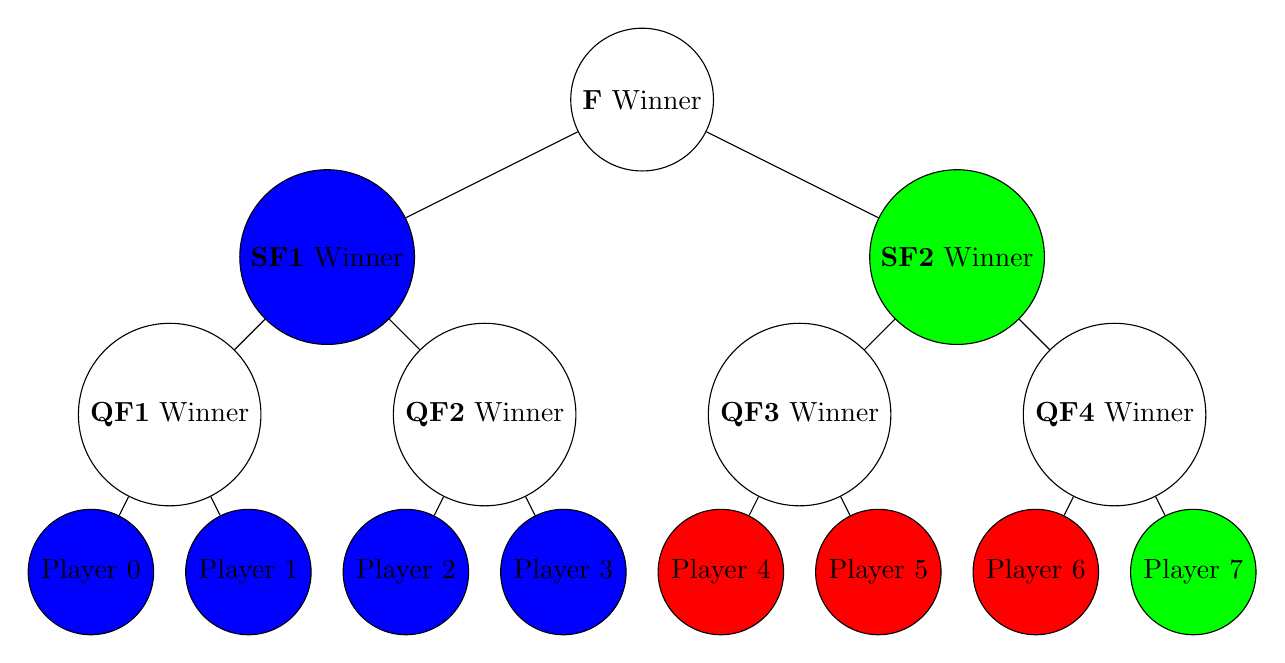
\begin{tikzpicture}[nodes={draw, circle}, -,  level distance=2cm, sibling distance=2cm]

    \node{\textbf{F} Winner}
      child { node[fill=blue]{\textbf{SF1} Winner}
              child{
                 node{\textbf{QF1} Winner}
                  child{node[fill=blue]{Player 0}}
                  child{node[fill=blue]{Player 1}}
                  }
                child [missing]
                child{
                  node{\textbf{QF2} Winner}
                    child{node[fill=blue]{Player 2}}
                    child{node[fill=blue]{Player 3}}
                    }
              }
      child [missing]
      child [missing]
      child [missing]
      child { node[fill=green]{\textbf{SF2} Winner}
              child{
                 node{\textbf{QF3} Winner}
                  child{node[fill=red]{Player 4}}
                  child{node[fill=red]{Player 5}}
                  }
                child [missing]
                child{
                  node{\textbf{QF4} Winner}
                    child{node[fill=red]{Player 6}}
                    child{node[fill=green]{Player 7}}
                    }
              };
\end{tikzpicture}
\caption{Tree Structure of a 3-round tournament illustrating the possible opponents (in blue)
of Player $7$ in the Final.}
\label{fig:tree}
\end{figure}

With the established model, one \textit{simply} needs to be able to predict the outcome of a match between
two players to be able to determine the outcome of a whole tournament.

\subsection{Variables}
\label{subsec:variables}
A tennis match opposes two players in a given environment.
For a given match, there also are bookmakers that determine betting odds.
These three agents have their own specificness. Some of the
characteristics can be analyzed without any context, some others not.
The firsts will be called \textit{intrisinc} while the latters
will be denoted as \textit{conditional}. For example, the favorite hand of a player
can be taken into account no matters their opponent while it makes no sense to take into account stats originating from matches
that are too different from the current one. These stats have to be chosen
conditionally to the current match.
A non-exhaustive list of determinant features can be found in Table~\ref{tab:features}.

\begin{table}
  \centering
  \begin{tabular}{|c|c|c|}
    \hline
    \textbf{Agents} & \textbf{Intrisinc Features} & \textbf{Conditional Features}\\
    \hline
    \multirow{5}{*}{Environment} & Surface & \\
      &  Date & \\
      & Weather & \\
      & Court & \\
      & Localisation &\\
      \hline
    \multirow{10}{*}{Players} & Identifier  & Aces per match \\
        &  Height/Weight  &  \%First serve \\
        & Ranking / Points & Double faults per match \\
        & Age & Previous matches against each other \\
        & Current Shape & \\
        & Hand & \\
        & W/L Streak & \\
        & Last Match & \\
        & Favorite Move & \\
        & Favorite Surface  & \\
    \hline
        Bookmakers & & Betting odds\\
    \hline
  \end{tabular}
  \caption{Non-exhaustive list of features with influence on the outcome of a tennis match.}
  \label{tab:features}
\end{table}

To make the problem independent from the players involved, in place
of directly taking into account the variables, one could rather work
with differences between the features of the two players.
As an example, in place of working with two \textit{ATP} points,
one could only consider the difference between them.

This way of doing offers another advantage. It can reduce up to a factor $2$
the number of input features related to players.

Another thing that could be imagined is to weight some of the variables beforehand.
As an example, one takes a match that opposes two players that have already been opposed in the past.
The stats of these previous matches should maybe have a larger importance than
the ones against common opponents and even more than general stats.


\section{Data Collection}
\subsection{Sources}
In Subsection~\ref{subsec:variables}, one listed determinant variables. Concerning the environment, one will have to
retrieve the information mainly from the tournament organisator and from
the weather forecast. Concerning the players features, one should have a look at the \textit{ATP} website.
And for the different betting odds, one can retrieve them from the different online gambling websites.
These sources are \textit{primary} sources. One could also find \textit{secondary} sources which could have
formatted the raw data made available by these \textit{primary} sources.
\subsection{Format} Either the data will be available in a usable formatting (\textit{e.g.} spreadsheets)
or in a non directly exploitable format (\textit{e.g.} web pages). In the second case, one can develop \textit{scraping} programs to extract the valuable data.
For this purpose, the \texttt{Python} language has a dedicated library called \texttt{BeautifulSoup}.
One advantage of web scraping is that it enables to format the value as needed.




\section{Model}
\subsection{Neural network}
Machine learning methods and more specifically artificial neural networks can be used to predict the outcome of a tennis match. Indeed, artificial neural networks are effective approach to solve real life classification problems.

Artificial neural network consists of several layers including an input layer, hidden layers with neurons and an output layer. To each connection in the network is associated a weight. Each neuron computes an output value from its inputs and its weights. This output value will be passed as the input value of other neurons.

The objective of the artificial neural network process is thus to find the set of weight values which provide  the appropriate output vector that will match the target values as well as possible.

In our case, the algorithm learn based on an input vector which consists of various characteristics of the players and the match built from historical data as well as an output value which correspond to the outcome of the match.

The major challenge of using this method is the problem of overfitting and the selection of the best hyperparameter.

Overfitting can occur due to a lack of data. The outcome of a future match will be estimated by means of characteristics of past matches. It is thus important that those matches occur on the same surface and with similar opponents in order to reflect in the best way the players’ performance. The training data will therefore be slightly restricted. The selection of the most relevant features has to be done carefully.

The result of the model will depend on the number of hidden layers as well as the number of neurons in each layer. One must thus select the appropriate hyperparameters carefully.  It can be done by adjusting the parameters to reduce the error up to an acceptable value.

\subsection{Markov chain}
%hard to solve analytically because of cycles?
%decomposing into points allow to have more data as there is more points played than matchs?
\paragraph{}
Markov chain allows to decompose the fact of winning a match into winning a point while serving or receiving. Deriving Markov chains is straight forward. Each state may lead to 2 other states depending on the winner of the point, those 2 other states are determined according to tennis' rules. The probabilities of each players winning the point depend on which player is currently serving. After having derived a model for winning a game, this model may be reused to derive the one modeling a set which in turn can be used to model a match. Once the Markov chain model is derived, probabilities of winning a match may be computed analytically or numerically by multiplying iteratively the initial probability distribution by the transition matrix to approximate the stationary distribution.
\paragraph{}
We may use the same probabilities the whole match based on the hypothesis that the points random variables are independent and identically distributed. This is not the case in practice as those probabilities may be influenced by other factors that evolve during the match as the player fatigue,... However those factors are likely to evolve the same way for both players, results obtained based on this hypothesis are thus likely to be close from reality even if not totally accurate. Another solution would be to adapt the probabilities of winning on serve according to those external factors that evolves with time. It allows to be closer to reality but complexify the model.

\begin{figure}[!h]
\begin{center}
\includegraphics[width = 10cm]{markov.png}
\caption{\label{markov} Markov chain representing a game, player A serving}
\end{center}
\end{figure}

\paragraph{}
%Je suis absolument pas sur de ce paragraphe, j'ai essayé de simplifier ce que j'ai compris des documents mais dans les documents ils partent dans des pages et des pages de stat.
An improvement of this method would be to dynamically adapt probabilities of winning a point according to what happened before during the match. However, we want to compute it before the match starts. Probabilities are computed for a given state, this state gives us information about what could have happened during the match (number of points won by a given player, ...). What could thus be done is to simulate the match with given probabilities and update the probabilities for a given state according to the outcome of the math if this particular state is reached.
%to how the match went if when and if it reaches this state.

\subsection{Support Vector Machine}
A support vector machine consists in mapping examples such as previous matches to points in space and finding a maximum-margin hyperplane which divides them into their labelled categories (e.g the win and lose categories). An unseen example can be mapped in the same space and will be classified according to the side of the margin to which it belongs.

\section{Model Verification}
Cross-validation \textit{per se} is not well-suited for prediction of events that are time-ordered.
One has to predict an upcoming match only based on past matches.
It is then possible to slightly adapt the method to preserve the required temporal order.
If the data for consecutive years is available, one can use the data of year $1$ to train
and then test on year $2$. One can then train the model on both years $1$ and $2$, and test on
year $3$. One proceeds in the same way for all the available years and obtains a estimation
of the model performance.

%\nocite{sipko}
%\nocite{imecs}
%\nocite{markov}
%\nocite{random_forest}
%\nocite{madurska}
%\nocite{bengtson}
%\nocite{barnett}
%\nocite{bunker}
%\printbibliography

\end{document}
